\documentclass[12pt,a4paper]{article}

% ── Packages ──────────────────────────────────────────────────────────────
\usepackage[margin=2.5cm]{geometry}
\usepackage{xcolor}
\usepackage{tikz}
\usetikzlibrary{arrows.meta, positioning, calc}
\usepackage{tcolorbox}
\tcbuselibrary{skins}
\usepackage{booktabs}
\usepackage{caption}
\usepackage{float}
\usepackage{parskip}

% ── Colour palette & Styles ───────────────────────────────────────────────
\definecolor{clrPurple}{HTML}{7F77DD}
\definecolor{clrPurpleLight}{HTML}{EEEDFE}
\definecolor{clrPurpleDark}{HTML}{3C3489}
\definecolor{clrTeal}{HTML}{1D9E75}
\definecolor{clrTealLight}{HTML}{E1F5EE}
\definecolor{clrTealDark}{HTML}{085041}
\definecolor{clrGray}{HTML}{888780}
\definecolor{clrGrayLight}{HTML}{F1EFE8}
\definecolor{clrGrayDark}{HTML}{444441}
\definecolor{clrBlue}{HTML}{378ADD}
\definecolor{clrBlueLight}{HTML}{E6F1FB}
\definecolor{clrBlueDark}{HTML}{0C447C}

\tcbset{
  sumbox/.style={
    enhanced, colback=clrGrayLight, colframe=clrGrayDark,
    fonttitle=\bfseries, title=#1, left=8pt, right=8pt, top=6pt, bottom=6pt, arc=4pt
  }
}

\tikzset{
  fsm state/.style={circle, draw, thick, minimum size=1.8cm, font=\small\bfseries, align=center},
  fsm idle/.style={fsm state, fill=clrGrayLight, draw=clrGrayDark},
  fsm calc/.style={fsm state, fill=clrPurpleLight, draw=clrPurpleDark},
  fsm done/.style={fsm state, fill=clrTealLight, draw=clrTealDark},
  reg box/.style={rectangle, draw=clrBlueDark, fill=clrBlueLight, minimum width=2.8cm, minimum height=0.8cm, font=\ttfamily\small, rounded corners=3pt},
  comb box/.style={rectangle, draw=clrPurpleDark, fill=clrPurpleLight, minimum width=3.5cm, minimum height=2cm, font=\small, align=center, rounded corners=3pt},
  arr/.style={-{Stealth[length=5pt]}, thick},
  darr/.style={-{Stealth[length=5pt]}, thick, dashed},
}

\begin{document}

\begin{center}
    {\LARGE\bfseries Summary: \texttt{isqrt} Hardware Module\par}
    \vspace{0.2cm}
    {\large A Hardware Implementation of the Integer Square Root\par}
    \vspace{0.4cm}
    {\color{clrGray}\rule{8cm}{0.5pt}\par}
\end{center}

% ════════════════════════════════════════════════════════════════════════
\section*{1. The Core Concept}
% ════════════════════════════════════════════════════════════════════════
The \texttt{isqrt} module calculates the integer square root of a 16-bit unsigned number ($q = \lfloor\sqrt{N}\rfloor$). The output is an 8-bit integer. Because the input is processed \textbf{two bits at a time} (from MSB to LSB), the calculation always takes \textbf{exactly 8 iterations}.

% ════════════════════════════════════════════════════════════════════════
\section*{2. The Finite State Machine (FSM)}
% ════════════════════════════════════════════════════════════════════════
The entire process is controlled by a 3-state machine. It waits for a signal, loops exactly 8 times to calculate the root, and then alerts the system when finished.

\begin{figure}[H]
\centering
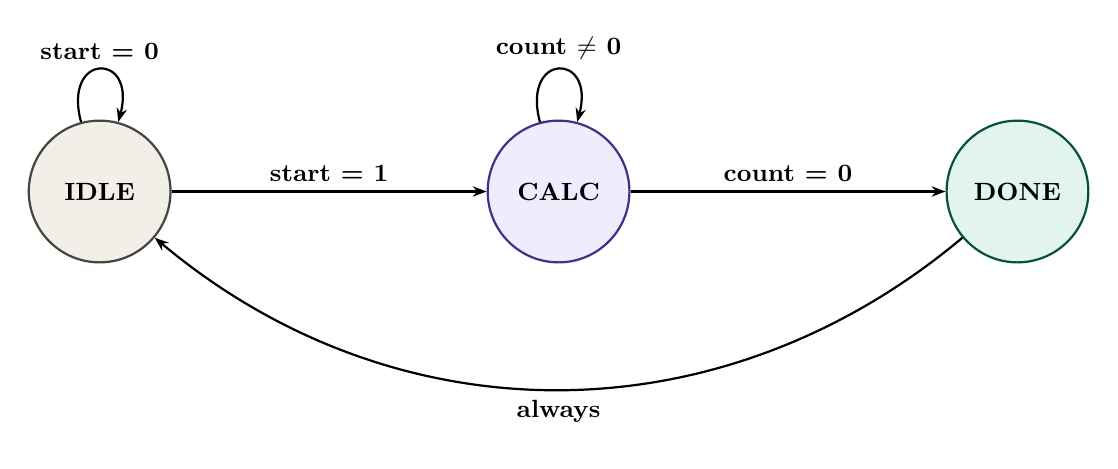
\begin{tikzpicture}[node distance=4cm]
  % States
  \node[fsm idle] (IDLE) {IDLE};
  \node[fsm calc, right=of IDLE] (CALC) {CALC};
  \node[fsm done, right=of CALC] (DONE) {DONE};

  % Transitions
  \draw[arr] (IDLE) -- (CALC) node[midway, above, font=\small\bfseries] {start = 1};
  \draw[arr] (CALC) -- (DONE) node[midway, above, font=\small\bfseries] {count = 0};
  \draw[arr] (DONE) to[bend left=40] node[midway, below, font=\small\bfseries] {always} (IDLE);
  
  \draw[arr] (CALC) to[loop above, looseness=5] node[above, font=\small\bfseries] {count $\neq$ 0} (CALC);
  \draw[arr] (IDLE) to[loop above, looseness=5] node[above, font=\small\bfseries] {start = 0} (IDLE);
\end{tikzpicture}
\caption*{Figure 1: The 3-State FSM controlling the computation.}
\end{figure}

% ════════════════════════════════════════════════════════════════════════
\section*{3. Datapath \& The Restoring Algorithm}
% ════════════════════════════════════════════════════════════════════════
The math relies on three registers interacting with a block of combinational logic. It uses a \textbf{restoring digit-recurrence} algorithm (similar to long division).

\begin{figure}[H]
\centering
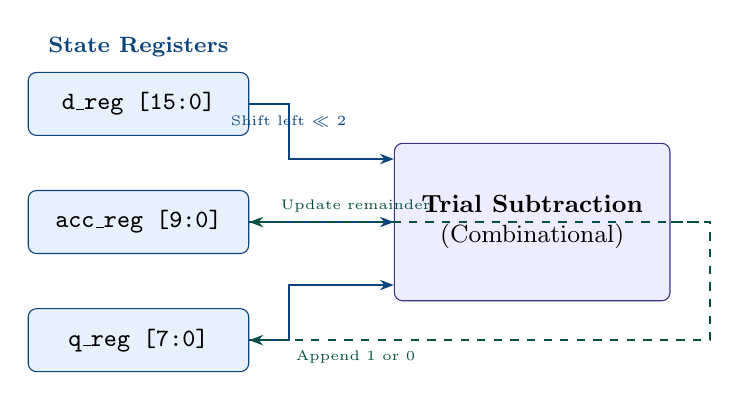
\begin{tikzpicture}
  % Registers
  \node[reg box] (dreg) at (0,3) {\texttt{d\_reg [15:0]}};
  \node[reg box] (areg) at (0,1.5) {\texttt{acc\_reg [9:0]}};
  \node[reg box] (qreg) at (0,0) {\texttt{q\_reg [7:0]}};
  
  \node[font=\footnotesize\bfseries\color{clrBlueDark}, above=2pt of dreg] {State Registers};

  % Combinational Logic
  \node[comb box] (comb) at (5, 1.5) {\textbf{Trial Subtraction}\\(Combinational)};
  
  % Arrows to Comb
  \draw[arr, clrBlueDark] (dreg.east) -- ++(0.5,0) |- ($(comb.west)+(0,0.8)$) node[pos=0.3, above, font=\tiny] {Shift left $\ll$ 2};
  \draw[arr, clrBlueDark] (areg.east) -- (comb.west);
  \draw[arr, clrBlueDark] (qreg.east) -- ++(0.5,0) |- ($(comb.west)+(0,-0.8)$);

  % Feedback Arrows
  \draw[darr, clrTealDark] (comb.east) -- ++(0.5,0) |- ($(areg.east)+(1.5,0)$) -- ++(-1.5,0) node[pos=0.1, above, font=\tiny] {Update remainder};
  \draw[darr, clrTealDark] (comb.east) -- ++(0.5,0) |- ($(qreg.east)+(1.5,0)$) -- ++(-1.5,0) node[pos=0.1, below, font=\tiny] {Append 1 or 0};
\end{tikzpicture}
\caption*{Figure 2: Simplified Datapath. Registers feed logic, which updates registers.}
\end{figure}

\begin{tcolorbox}[sumbox={How the iteration works (CALC state)}]
  Every clock cycle, the module tests whether the next bit of the answer is a 1 or a 0 by performing a \textbf{trial subtraction}:
  \begin{itemize}\setlength\itemsep{0pt}
      \item \textbf{Combine:} Grabs the next 2 bits of the shifted \texttt{d\_reg} and appends them to \texttt{acc\_reg}.
      \item \textbf{Test:} Subtracts a "trial divisor" (based on \texttt{q\_reg}) from this combined remainder.
      \item \textbf{Pass (Result $\ge$ 0):} The subtraction is kept; append \textbf{1} to the quotient.
      \item \textbf{Fail (Result $<$ 0):} The subtraction is discarded (restored); append \textbf{0} to the quotient.
  \end{itemize}
\end{tcolorbox}

% ════════════════════════════════════════════════════════════════════════
\section*{4. Timing and Performance}
% ════════════════════════════════════════════════════════════════════════
Because the algorithm runs step-by-step alongside the clock, the performance is highly predictable. 

\begin{center}
\begin{tabular}{@{}ll@{}}
\toprule
\textbf{Phase} & \textbf{Clock Cycles} \\
\midrule
Enter IDLE / Latch Input  & 1 cycle \\
Execute CALC logic & 8 cycles \\
Enter DONE / Latch Output & 1 cycle \\
\midrule
\textbf{Total Latency} & \textbf{10 cycles} \\
\bottomrule
\end{tabular}
\end{center}

At a standard clock speed of 100 MHz (10 ns per cycle), the total time to compute any square root is precisely \textbf{100 nanoseconds}.

\end{document}